%\documentclass[draft]{ws-procs9x6}
\documentclass{ws-procs9x6}

\begin{document}

\title{Stable Cliff Climbing for Hexapod Robot with Articulated Body}

\author{A. V. Panchenko$^*$ and V. E. Pavlovsky$^{**}$}

\address{Faculty of Mechanics and Mathematics, Lomonosov Moscow State University,\\
Moscow, 119991, Russia\\
$^*$E-mail: PanchenkoAV@vap.ru\\
$^{**}$E-mail: vlpavl@mail.ru}

\begin{abstract}
The paper describes kinematic control for hexapod robot with three segments articulated body. Forward and inverse kinematics for articulated body described. Static stability studied in case of climbing the so--called cliff obstacle. Conditions for static stability during climbing sequence provided.
\end{abstract}

\keywords{Multi--legged robot; obstacle climbing; articulated body; simulation.}

\bodymatter

\section{Introduction}\label{aba:intoduction}
Study of walking machines is rather old question. Starting in 
Ancient China primitive mechanical designs\cite{yan2005historical} and ending with state of the art reinforcement learning \cite{peng2017deeploco} and model predictive control approaches\cite{diedam2008online}. Multi--leged walking robots are complicated systems in terms of control and planning due to significant number of degrees of freedom (d.o.f.) and actuators, complexity of the environment and etc. Nowadays the most complex and robust walking machines are made by Boston Dynamics company\cite{raibert2008bigdog}. Its robots are capable of working in human environment and outdoors. The basis of their solution is model predictive control and non-linear optimization. Their robots are based on the kinematics of mammals - dogs or horses. The kinematics of hexapod robots in turn is based on insects and spiders.

The main idea of the article – to study robot with articulated body, that differs from conventional mainstream hexapods have rigid body with legs attached symmetrically. This arrangement has its limitations but still can be surprisingly agile and overcomes complex obstacles as it was demonstrated in articles\cite{golubev2008control,golubev2009motion,golubev2013motion}. Introducing additional degrees of freedom – making multiple rigid segments to be a body instead of one rigid body segment increases robot’s geometric patency. On the other hand there is going to be trade off – the complexity of control will increase\cite{panchenko2016control} along with number of d.o.f. and actuators but the robot will climb up higher obstacles or do maneuvers that robots with rigid body are not capable of. For example, go through narrow passage, sharp ditch and windrows.

%The class file loads the packages {\tt amsfonts, amsmath, amssymb,
%chapterbib, cite, dcolumn, epsfig, rotating} and {\tt url} at
%startup. Please try to limit your use of additional packages as they
%often introduce incompatibilities. This problem is not specific to
%the WSPC styles; it is a general \LaTeX{} problem. Check this
%article to see whether the required functionality is already
%provided by the WSPC class file. If you do need additional packages,
%send them along with the paper. In general, you should use standard
%\LaTeX{} commands as much as possible.

\section{Robot Kinematics}
Let us consider robot depicted on figure Fig. \ref{aba:robot_1}. It has six so-called insectomorphic legs, i.e. insect-like leg kinematics. Each leg has three degrees of freedom. Body consists of three rigid segments connected with hinges to each other. Body that consists of several segments connected to each other with controllable joints and can change its geometry is called articulated.

\begin{figure}
  \begin{center}
    \psfig{file=pics/robot_2.eps,width=2in}
  \end{center}
  \caption{Hexapod robot with articulated body.}
  \label{aba:robot_1}
\end{figure}

The total number of degrees of freedom (d.o.f.) for specified robot is 26:
\begin{itemlist}
      \item	3 d.o.f. for each leg, i.e. 18 d.o.f. for all legs;
      \item 2 d.o.f. for body segments;
      \item	6 d.o.f. for the whole system as one single body.
\end{itemlist}
Overall it is 26 d.o.f. and 20 of them can be controlled with an actuators installed in corresponding rotational joints. Leg kinematics is well known and was already studied in all details.


%In order to facilitate our processing of your article, please give
%easily identifiable structure to the various parts of the text by
%making use of the usual \LaTeX{} commands or by using your own commands
%defined in the preamble, rather than by \hbox{using} explicit layout
%commands, such as \verb|\hspace, \vspace, \large, \centering|,
%etc.~Also, do not redefine the page-layout parameters.~For more
%information on layout and font specifications, please refer to our
%\verb|Layout and| \verb|Font Specification Guide|.

\section{Cliff Obstacle}
Cliff obstacle consists of three planes two of which are horizontal and one is vertical as depicted on Fig. \ref{aba:cliff}.


\begin{figure}
  \begin{center}
    \psfig{file=pics/cliff.eps,width=2.5in}
  \end{center}
  \caption{Cliff obstacle.}
  \label{aba:cliff}
\end{figure}

The distance between two horizontal planes is equal to $H$. Robot starts from the lower horizontal plane and his goal is to climb up the higher horizontal plane using only the Coulomb friction.
To overcome cliff obstacle robot moves using so-called gallop gait when a pair of symmetrical legs from left and right sides of the robot are in transition state and the others are in support state, i.e. in every moment of time there are four legs in contact with obstacle. Body kinematics will be considered in next section.

%User defined macros should be placed in the preamble of the article,
%and not at any other place in the document. Such private
%definitions, i.e. definitions made using the commands
%\verb|\newcommand,| \verb|\renewcommand,| \verb|\newenvironment| or
%\verb|\renewenvironment|, should be used with great care. Sensible,
%restricted usage of private definitions is encouraged. Large macro
%packages and definitions that are not used in this example article
%should be avoided. Please do not change the existing environments,
%commands and other standard parts of \LaTeX.

\section{Body Kinematics}
Robot’s body consists of three equal rigid segments connected to each other with rotational joints with axes aligned in lateral direction of the body. Each segment has a pair of legs connected. Additional joints with angles $\delta_1$ and $\delta_2$ in the robots body allow to bend body and follow the surface shape and shift legs mounting points towards to supporting surface. 
The following procedure is defined to calculated body joint angles. Initial and goal poses for middle segment are connected with a cubic spline curve, which represents target trajectory for middle segment. If segments and their trajectory are known then the task is solved through simple linear approximation as depicted on Fig. \ref{aba:spline}.

\begin{figure}
  \begin{center}
    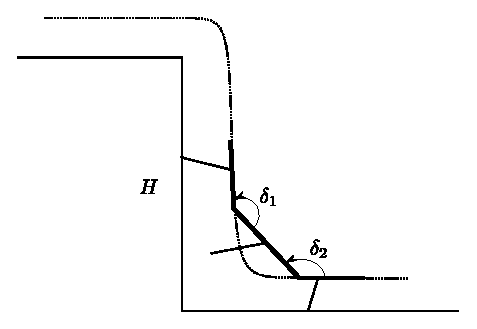
\psfig{file=pics/spline.eps,width=2in}
  \end{center}
  \caption{Body inverse kinematics through simple linear approximation.}
  \label{aba:spline}
\end{figure}

To keep the contact points on the goal trajectory all joints should act in a coordinated way. At every moment of time all joint coordinates must be updated to keep the end effectors at the goal position. Additional mobility inside the robots body should be taken into account because all legs are connected to the different segments.  Target point $\overline{R}_i$ for $i$-th leg is given in global reference frame. To obtain leg joint angles the inverse kinematic equations are used, point $\overline{R}_i$ must be translated into leg’s reference frame. To manage all relative coordinate transformations of shifts and rotations between body segments, legs and joints, homogeneous coordinates are used. Calculation of all coordinate transformation for each leg at every moment of time can be easily done automatically through well-known kinematics of a robot.
The main differences of articulated body from single segment body are:
\begin{itemlist}
  \item Higher ability to overcome obstacles –-- segments follow the surface;
  \item Articulated body is able to shift mounting points of its legs –-- service region is not constant, i.e. in some conditions robot can reach contact surface and put legs on it;
  \item Center of gravity is shifted in a wider range with all else parameters being equal –-- critical parameter in static stability preservation in extreme conditions.
\end{itemlist}

%You can obtain these files from the following website:
%\url{http://eproceedings.worldscinet.com/authors.shtml},
%\url{http://www.wspc.com.sg/style/proceedings_style.shtml} and
%\url{http://www.icpress.co.uk/authors/stylefiles.shtml#proceedings}.

\section{Cliff Climbing Stability}
The system is stable when sums of all external forces and all momentums are equal to zero. 

\begin{equation}
  \left\{
    \begin{array}{cc}
    \sum\limits^N_{i=1}\overline{R}_i + \overline{P} = 0\\
    \sum\limits^N_{i=1}[\overline{r}_i\times\overline{R}_i] + [\overline{r}_c\times\overline{R}_c] = 0\\
    \end{array}
  \right.
  \label{eq:eq1}
\end{equation}

  
The following configurations of supporting legs displacement should be studied for static stability:
\begin{itemlist}
  \item All legs on some horizontal plane. This case is already well studied;
  \item Front legs lean against the vertical plane and rear legs stand on the lower horizontal plane. Let us numerate this configuration as Number One.
  \item Front legs are placed at the upper horizontal plane, while the rear legs stand on the vertical plane. Let us numerate this configuration as Number Two.
  \item All legs stand on the upper horizontal plane –-- this case is similar to the initial one.
\end{itemlist}
  
  Considering the robot as a slow moving system at every moment of time let us find conditions for static stability. 
  Reference frame Oxyz is defined as depicted on Fig. \ref{aba:configuration_1}.

\subsection{First Configuration}

\begin{figure}
  \begin{center}
    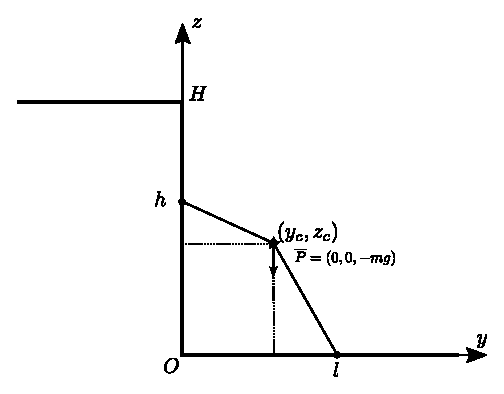
\psfig{file=pics/configuration_1.eps,width=2in}
  \end{center}
  \caption{First static configuration.}
  \label{aba:configuration_1}
\end{figure}

Contact points of the legs for first configuration are as follows:
\begin{equation}
  \begin{array}{l}
    \overline{r}_1 = (d,0,h),
    \overline{r}_2 = (-d,0,h),
    \overline{r}_3 = (d,l,0),
    \overline{r}_4 = (-d,l,0).
  \end{array}
\end{equation}

There is a reaction $\overline{R}_i$ acting on the robots legs at each contact point:

\begin{equation}
\overline{R}_i =  N_i\cdot\overline{n}_i+F^i_\tau\cdot\overline{\tau}_i+F^i_\nu\cdot\overline{\nu}_i
\end{equation}

The $\overline{\tau}_i$ and $\overline{nu}_i$ vectors have the following coordinates:

\begin{equation}
\begin{array}{ccc}
  \overline{n}_1 = (0,1,0), & \overline{\tau}_1 = (0,0,1),& \overline{\nu}_1 = (1,0,0),\\
  \overline{n}_2 = (0,1,0), & \overline{\tau}_2 = (0,0,1),& \overline{\nu}_2 = (1,0,0),\\
  \overline{n}_3 = (0,0,1), & \overline{\tau}_3 = (0,1,0),& \overline{\nu}_3 = (1,0,0),\\
  \overline{n}_4 = (0,0,1), & \overline{\tau}_4 = (0,1,0),& \overline{\nu}_4 = (1,0,0).\\
\end{array}
\end{equation}

The center of gravity has coordinates:
\begin{equation}
  \overline{r}_c = (0,y_c,z_c)\\
\end{equation}

The gravity force $\overline{P}$ acts on the center of gravity of the robot:

\begin{equation}
\overline{P} = (0,0,-P)
\end{equation}

The equations of static stability for first configuration are as follows:

\begin{equation}
\label{eq:case1_initial}
\left\{
  \begin{array}{rcl}
    F_\nu^1 + F_\nu^2 + F_\nu^3 + F_\nu^4 &=& 0, \\
    N_1 + N_2 + F_\tau^3 + F_\tau^4 &=& 0, \\
    F_\tau^1 + F_\tau^2 + N_3 + N_4 &=& P, \\
    N_1h + N_2h + Py_c &=& l(N_3 + N_4), \\
    d(F_\tau^1 + N_3) &=& F_\tau^2d + F_\nu^1h + F_\nu^2h + N_4d, \\
    d(F_\tau^3 + N_1) &=& F_\tau^4d + N_2d +F_\nu^3l + F_\nu^4l.\\
  \end{array}
\right.
\end{equation}

The total number of equation is six. The number of unknown variables is twelve. Let us assume that the friction forces are modelled with Coulomb mathematical model:

$F_j^i = k_j^i\cdot N_i$, where $k_j^i$ is coefficient of friction for $i$-th leg in $j$-th direction.

After substitution of the Coulomb friction model, the Eq. (\ref{eq:case1_initial}) will transform into the following system:

\begin{equation}
\label{eq:case1_subs_kulon}
\left\{
\begin{array}{rcl}
  N_1k_\nu^1 + N_2k_\nu^2 + N_3k_\nu^3 + N_4k_\nu^4 &=& 0,\\
  N_1 + N_2 + N_3k_\tau^3 + N_4k_\tau^4 &=& 0, \\
  N_3 + N_4 + N_1k_\tau^1 + N_2k_\tau^2 &=& P, \\
  N_1h + N_2h + Py_c &=& l(N_3 + N_4), \\
  d(N_3 + N_1k_\tau^1) &=& dN_4 + dN_2k_\tau^2 + hN_1k_\nu^1 + hN_2k_\nu^2,\\
  d(N_1 + N_3k_\tau^3) &=& dN_2 + dN_4k_\tau^4 + lN_3k_\nu^3 + lN_4k_\nu^4\\
\end{array}
\right.
\end{equation}

The number of unknowns variables remains the same, and besides $N_i >~0$. Let us introduce additional assumptions that the left and the right side of the robot are loaded equally and coefficients of friction are the same between left and right legs:

\begin{equation}
\label{eq:case1_assumptions_1_and_2}
\left\{
\begin{array}{rcccl}
    k_\nu^1  &=& -k_\nu^2&=& k_\nu,\\
    k_\nu^3  &=& -k_\nu^4&=& k_\nu,\\
    k_\tau^1 &= &k_\tau^2&=& k_\tau^u,\\
    k_\tau^3 &= &k_\tau^4&=& k_\tau^d,\\
    N_1 &=& N_3 &=& N_u, \\
    N_2 &=& N_4 &=& N_d. \\
\end{array}
\right.
\end{equation}

The system of three equations and four variables obtained:

\begin{equation}
\label{eq:case1_subs_assumptions_1_and_2}
\left\{
\begin{array}{rcl}
  N_u + N_dk_\tau^d &=& 0, \\
  2N_d + 2N_uk_\tau^u &=& P, \\
  2hN_u + Py_c &=& 2lN_d.\\
\end{array}
\right.
\end{equation}
  
Number of unknowns is still greater than number of equations. One more assumption must be introduced:

\begin{equation}
  \label{eq:case1_assumption_3}
  k_\tau^u = k_\tau^d = k_\tau > 0
\end{equation}

Finally, the system of three equations and three unknowns obtained:

\begin{equation}
\label{eq:case1_final_system}
\left\{
\begin{array}{rcl}
  N_u &=& N_dk_\tau,\\  
  2N_d + 2N_uk_\tau &=& P,\\
  2hN_u + Py_c &=& 2lN_d.\\
\end{array}
\right.
\end{equation}

Let us find unknown reactions $N_u,N_d$ and $k_\tau$. From first and second equations of Eq. (\ref{eq:case1_final_system}) follows:

\begin{equation}
\label{eq:case1_Nu_and_Nd}
\begin{array}{rcl}
  N^u &=& N^dk_\tau,\\
  N^d &=& \dfrac{P}{2(1+k_\tau^2)}.\\
\end{array}
\end{equation}

After substituting Eq. (\ref{eq:case1_Nu_and_Nd}) to the third equation of Eq. (\ref{eq:case1_final_system}) we have quadratic equation relative to $k_\tau$:

\begin{equation}
\label{eq:case1_k}
y_ck_\tau^2+hk_\tau + (y_c-l) = 0
\end{equation}

There are two solutions for quadratic Eq. (\ref{eq:case1_k}), but only one satisfies condition $0<k_\tau<1$:

\begin{equation}
\label{eq:case1_k12}
\begin{array}{rcl}
 0 < k_\tau &=& -\dfrac{h - \sqrt{h^2 - 4y_c^2 + 4ly_c}}{2y_c} < 1\\
\end{array}
\end{equation}


%\begin{verbatim}
%\documentclass{ws-procs9x6}
%\begin{document}
%\title{FOR PROCEEDINGS CONTRIBUTORS: ...}
%\author{A. B. AUTHOR$^*$ and C. D. AUTHOR}
%\address{University Department, ...}
%\begin{abstract}
%This article explains how to ...
%\end{abstract}
%\keywords{Style file; \LaTeX, ...}
%\bodymatter
%\section{Using Other Packages}
%The class file has ...
%\bibliographystyle{ws-procs9x6}
%\bibliography{ws-pro-sample}
%\end{document}
%\end{verbatim}

\subsubsection{Dimensionless parameters}

It is easy to see that the Eq. (\ref{eq:case1_k12}) for $k_\tau$ depends on $l$,$h$ and $y_c$ parameters that are measured in meters – they all have the same physical dimension. Let us use this circumstance and define the following dimensionless parameters:

\begin{equation}
\label{eq:case1_dimesionless}
p_1 := \dfrac{h}{y_c},~p_2 := \dfrac{l}{y_c},~where ~y_c \ne 0.
\end{equation}

After solving Eq.~(\ref{eq:case1_k12}) with substituted Eq.~(\ref{eq:case1_dimesionless}), the solution of Eq.~(\ref{eq:case1_k12}) is depicted on Fig.~\ref{aba:case1_dimless_figure}.


\begin{figure}
  \begin{center}
    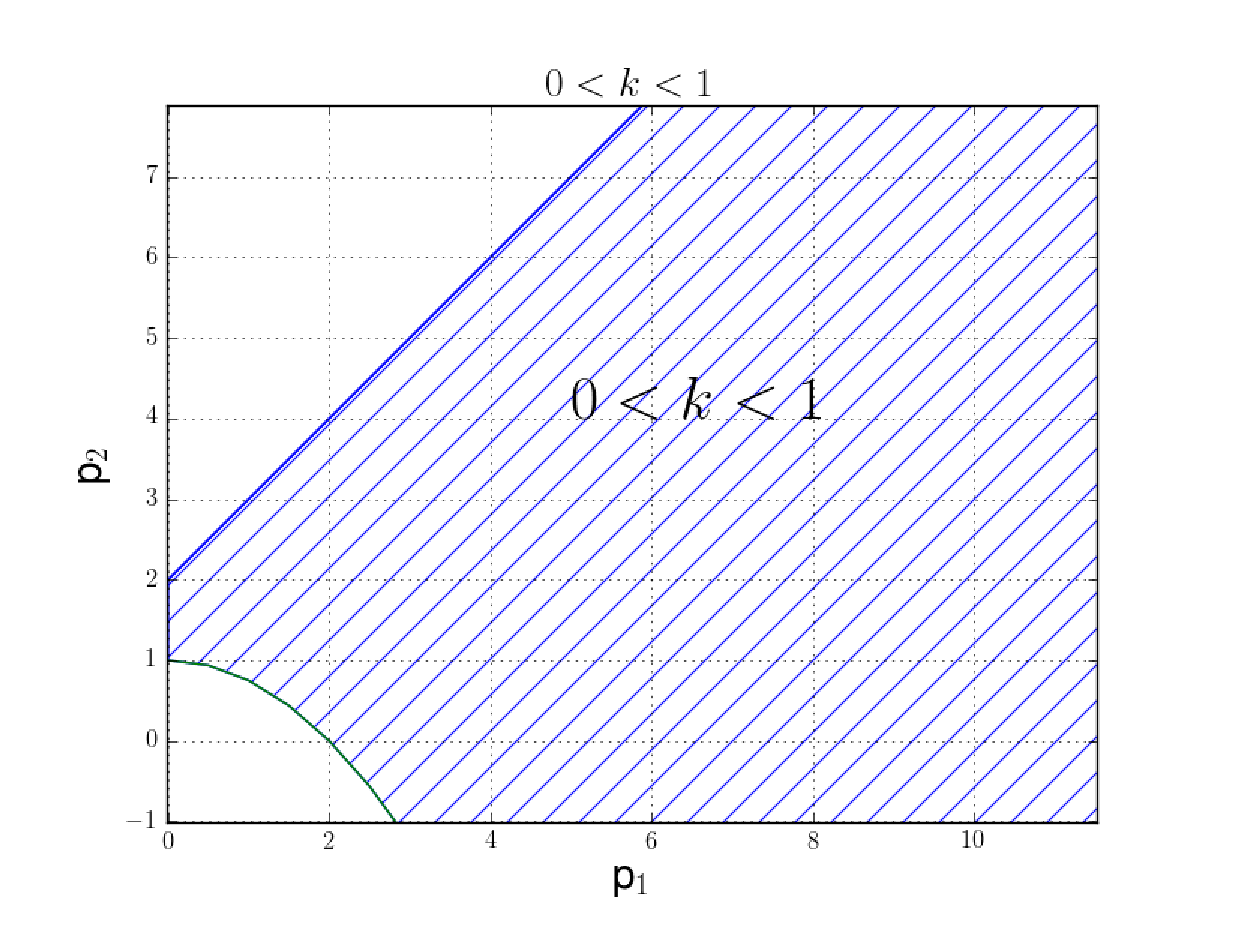
\psfig{file=pics/figure_1.eps,width=2.5in}
  \end{center}
  \caption{Solution of Eq. (\ref{eq:case1_k12}) with labeled contour lines for $k_\tau$ as a function of $(p_1, p_2)$.}
  \label{aba:case1_dimless_figure}
\end{figure}

From Fig. \ref{aba:case1_dimless_figure} it becomes clear that if there is lack of friction in contact points the robot should:
\begin{itemlist}
\item move its center of gravity closer to the rear legs;
\item choose contact points higher on the vertical plane for front legs;
\item choose contact points closer to vertical plane for rear legs.
\end{itemlist}

\subsection{Second Configuration}

Leg contact points for the second configuration are:
\begin{equation}
\label{eq:step_points_phase_2}
\begin{array}{rccccl}
  \overline{r}_1 &=& (d, l, H) , &\overline{r}_2 &=& (-d, l, H) \\
  \overline{r}_3 &=& (d, 0, h) , &\overline{r}_4 &=& (-d, 0, h) \\
\end{array}, where~l<0,H>h,y_c>l.
\end{equation}

Similarly, for the second configuration we get the following system of three equations:

\begin{equation}
\label{eq:case2_final_equations}
\left\{
\begin{array}{rcl}
N_u - N_dk_\tau &=& 0,\\
2N_u + 2N_d k_\tau &=& P,\\
2 N_d h + P y_c &=& 2 N_u (l + H k_\tau)\\
\end{array}
\right.
\end{equation}

There are two possible solutions for $k_\tau$, but only one meets requirement $0<k_\tau<1$:

\begin{equation}
  \label{eq:case2_k12}
 0 < k_\tau = \dfrac{(H-h) - \sqrt{(H-h)^2 - 4y^2_c + 4ly_c}}{2y_c} < 1
\end{equation}


\subsubsection{Dimensionless parameters}
Let us find solution of inequality $0<k_\tau<1$ using the following dimensionless parameters:

\begin{equation}
\label{eq:case2_dimentionless}
  p_1 := \dfrac{(H-h)}{y_c}, p_2 := \dfrac{l}{y_c}, where~y_c \ne 0.
\end{equation}

The solution of Eq. (\ref{eq:case2_k12}) is depicted on Fig. \ref{aba:case2_dimless_figure}.


\begin{figure}
  \begin{center}
    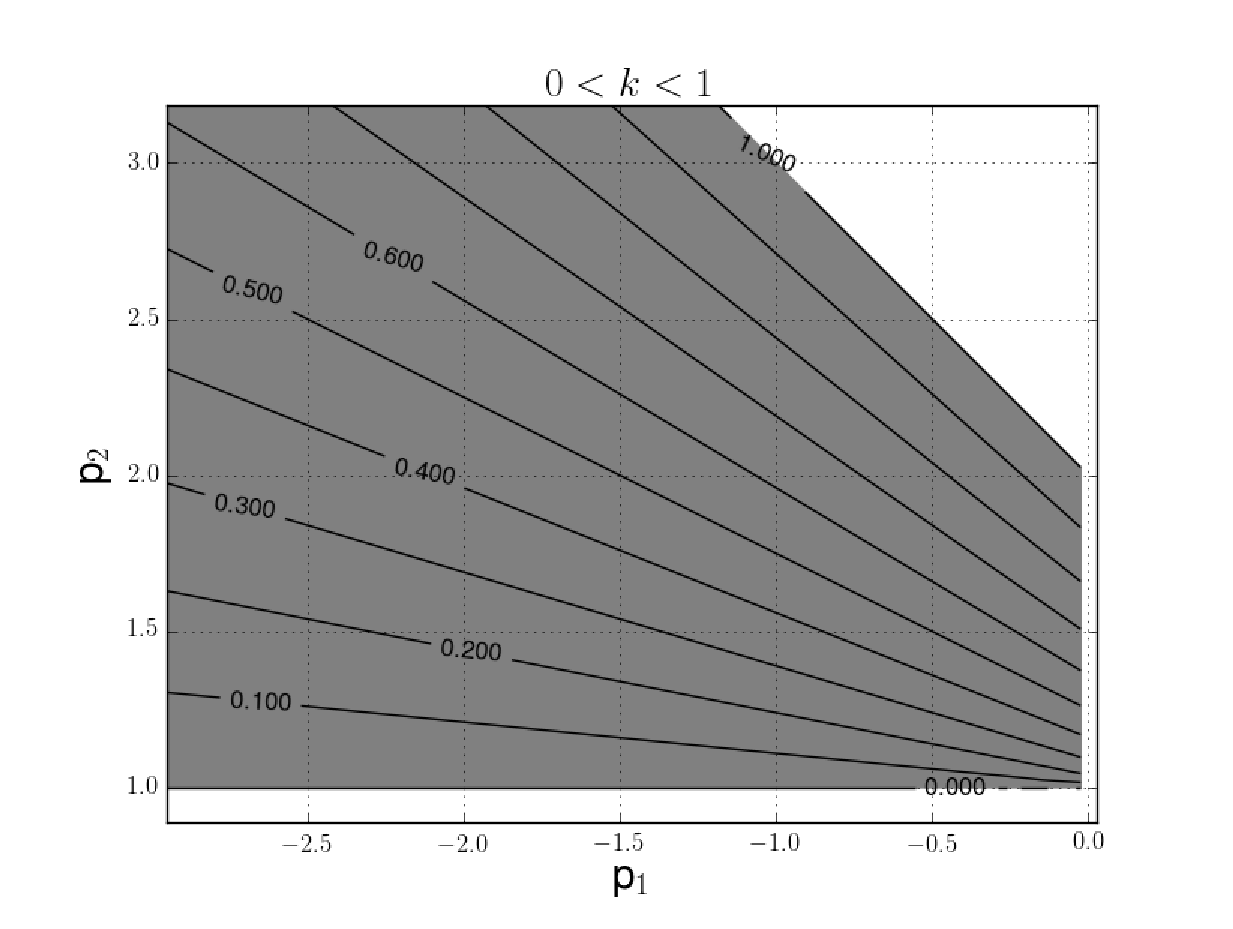
\psfig{file=pics/figure_2_2.eps,width=2.1in}
    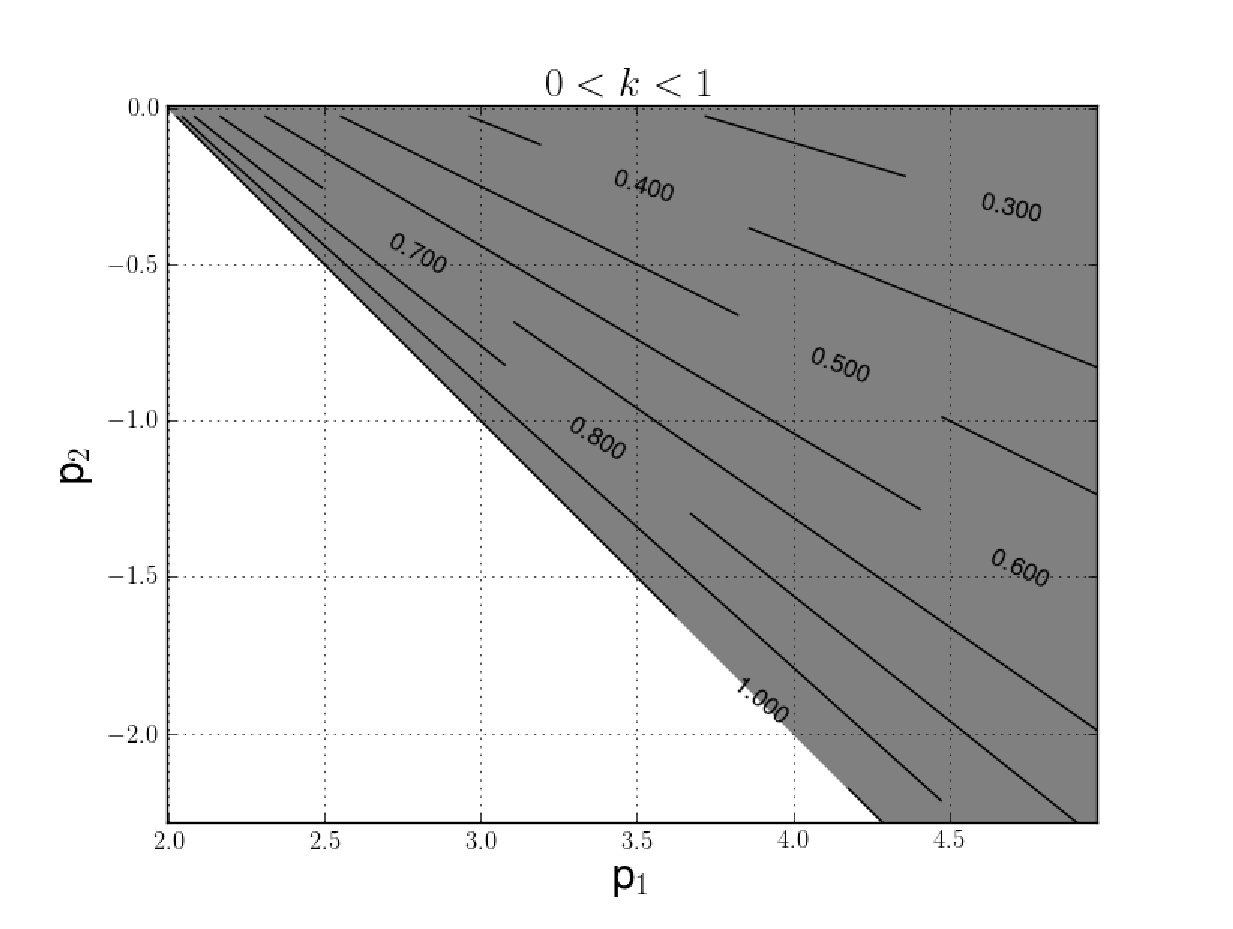
\psfig{file=pics/figure_2_1.eps,width=2.1in}
  \end{center}
  \caption{Solution of Eq. (\ref{eq:case2_k12}). Left - $y_c<0$, right - $y_c>0$.}
  \label{aba:case2_dimless_figure}
\end{figure}

From Fig. \ref{aba:case2_dimless_figure} it can be shown that for case when $y_c>0$ to reduce the value of $k_\tau$ robot should:
\begin{itemlist}
\item keep its center of gravity far from front legs;
\item keep rear legs as low as possible;
\item keep front legs closer to cliff edge.
\end{itemlist}

From Fig. \ref{aba:case2_dimless_figure} it can be shown that for case when $y_c<0$ to reduce the value of $k_\tau$ robot should:
\begin{itemlist}
  \item keep its center of gravity closer to front legs;
  \item keep rear legs as low as possible;
  \item keep front legs closer to cliff edge.
\end{itemlist}

In Eq. (\ref{eq:case2_dimentionless}) we have considered substitution in assumption that $y_c\ne0$. Let us see what happens when center of gravity is right above the cliffs edge in second configuration.

\subsubsection{Second configuration. $y_c$ equals to zero}
If the $y_c = 0$ the equations of static stability Eq. (\ref{eq:case2_final_equations}) will transform into the following system:

\begin{equation}
\label{eq:case2_zero_yc}
\left\{
\begin{array}{lcl}
  N_d - N_uk_\tau &=& 0 \\
  2N_u+2N_dk_\tau &=& P \\
  N_dh - N_ul &=& HN_uk_\tau\\
\end{array}
\right.
\end{equation}

There is only one solution for $k_\tau, N_u$ and $N_d$ for Eq. (\ref{eq:case2_zero_yc}):

\begin{equation}
\label{eq:case2_zero_yc_solution}
\left\{
\begin{array}{lcl}
  k_\tau &=& -\dfrac{l}{H-h},\\
  N_u &=& \dfrac{P(H-h)^2}{2((H-h)^2+l^2)}\\
  N_d &=& \dfrac{-Pl(H - h)}{2((H-h)^2+l^2)}\\
\end{array}
\right.
\end{equation}

Due to Eq. (\ref{eq:step_points_phase_2}) the Eq. (\ref{eq:case2_zero_yc_solution}) for $k_\tau$ is always greater than zero. From the other side, the requirement $k_\tau<1$ is equivalent to the following inequality:

\begin{equation}
\label{eq:case2_conditions_solution}
  0<-l<(H-h),where~l<0
\end{equation}

Equation (\ref{eq:case2_conditions_solution}) means that to provide stable configuration in case when $y_c=0$ the contact points should be chosen in a way, that the front legs should be closer to cliff edge than the rear legs.


\section{Hexapod simulation for cliff climbing}
To verify the static stability conditions the computer simulation of articulated hexapod was made.  The "Universal Mechanism"\cite{um} software package was used to provide dynamical model of the articulated hexapod robot and the cliff obstacle. All robot's legs have so called viscous elastic point contact models with the cliff obstacle.

\begin{figure}
  \centering
  \psfig{file=pics/kino_1.eps,width=1.5in}
  \psfig{file=pics/kino_2.eps,width=1.5in}\\
  \psfig{file=pics/kino_3.eps,width=1.5in}
  \psfig{file=pics/kino_4.eps,width=1.5in}\\
  \psfig{file=pics/kino_5.eps,width=1.5in}
  \psfig{file=pics/kino_6.eps,width=1.5in}\\
  \psfig{file=pics/kino_7.eps,width=1.5in}
  \psfig{file=pics/kino_8.eps,width=1.5in}\\
  \psfig{file=pics/kino_9.eps,width=1.5in}
  \psfig{file=pics/kino_10.eps,width=1.5in}\\
  \caption{Climbing motion sequence (left-to-right, top-to-bottom).
    \label{kinogramm}}
\end{figure}

The desired robot motion was manually scripted as list of scheduled commands for leg's positions and body configuration along with position and orientation. Robot's climbing motion sequence during simulation is depicted on Fig. \ref{kinogramm}. The resulting time of climbing maneuver in quasi static regime of motion takes about 50 seconds to climb up the cliff. The ratio between real and simulation time is approximately equal to 1 on computer with Core-i7 CPU and GTX950M GPU.


\section{Conclusion}
The analysis of robot's configurations in different poses on the cliff proved that stable quasi static motion is possible for all steps, i.e. the robot is capable of climbing the cliff with static stability preservation using only Coulomb friction forces. Articulated three segment body has shown advantages in comparison with similar rigid body in context of extreme obstacle overcoming. On the other hand, increased passability requires more complex motion planning and control.
Conditions for statics stability for all main climbing configurations obtained.


\section*{Acknowledgements}
The research work is supported by the Russian Foundation for Basic Research. The unique project number is 16--31--00524~mol\_a.



%\section{Sectional Units}
%Sectional units are obtained in the usual way, i.e. with the \LaTeX{}
%commands \verb|\section|, \verb|\subsection|,
%\verb|\subsubsection| and \verb|\paragraph|.
%
%\section{Section}
%This is just an example.
%
%\subsection{Subsection}
%This is just an example.
%
%\subsubsection{Subsubsection}
%This is just an example.
%
%\paragraph{Paragraph}
%This is just an example.
%
%\section*{Unnumbered Section}
%Unnumbered sections can be obtained by using \verb|\section*|.
%
%\section{Lists of Items}
%Lists are broadly classified into four major categories that can
%randomly be used as desired by the author:
%\begin{alphlist}[(d)]
%\item Numbered list.
%\item Lettered list.
%\item Unnumbered list.
%\item Bulleted list.
%\end{alphlist}
%
%\subsection{Numbered and lettered list}
%
%\begin{arabiclist}[(5)]
%\item The \verb|\begin{arabiclist}[]| command is used for the arabic
%number list (arabic numbers appearing within parenthesis), e.g.,
%(1), (2), etc.
%
%\smallskip
%
%\item The \verb|\begin{romanlist}[]| command is used for the roman
%number list (roman numbers appearing within parenthesis), e.g., (i),
%(ii), etc.
%
%\smallskip
%
%\item The \verb|\begin{Romanlist}[]| command is used for the cap roman
%\hbox{number list} (cap roman numbers appearing within parenthesis),
%e.g., (I), (II), etc.
%
%\smallskip
%
%\item The \verb|\begin{alphlist}[]| command is used for the alphabetic
%list (alphabets appearing within parenthesis),
%e.g., (a), (b), etc.
%
%\smallskip
%
%\item The \verb|\begin{Alphlist}[]| command is used for the cap
%alphabetic list (cap alphabets appearing within parenthesis),
%e.g., (A), (B), etc.
%\end{arabiclist}
%Note: For all the above mentioned lists (with the exception of
%alphabetic list), it is obligatory to enter the last entry's number
%in the list within the square bracket, to enable unit alignment.
%
%\subsection{Bulleted and unnumbered list}
%
%\begin{enumerate}
%\item[] The \verb|\begin{itemlist}| command is used for the bulleted list.
%
%\smallskip
%
%\item[] The \verb|\begin{unnumlist}| command is used for creating the
%  unnumbered list with the turnovers hangindent by 1\,pica.
%\end{enumerate}
%
%Lists may be laid out with each item marked by a dot:
%\begin{itemlist}
%\item item one
%\item item two
%\item item three.
%\end{itemlist}
%
%Items may also be numbered with lowercase Roman numerals:
%\begin{romanlist}[(iii)]
%\item item one
%\item item two
%    \begin{alphlist}[(a)]
%    \item lists within lists can be numbered with lowercase Roman letters
%    \item second item.
%    \end{alphlist}
%\item item three
%\item item four.
%\end{romanlist}
%
%\section{Theorems and Definitions}
%\noindent{\bf Input:}
%
%\begin{verbatim}
%\begin{theorem}
%We have $\# H^2 (M \supset N) < \infty$ for an inclusion ...
%\end{theorem}
%\end{verbatim}
%
%\noindent{\bf Output:}
%
%\begin{theorem}
%We have $\# H^2 (M \supset N) < \infty$ for an inclusion $M \supset
%N$ of factors of finite index.
%\end{theorem}
%
%\noindent{\bf Input:}
%
%\begin{verbatim}
%\begin{theorem}[Longo, 1998]
%For a given $Q$-system...
%\[
%N = \{x \in N; T x = \gamma (x) T, T x^* = \gamma (x^*) T\},
%\]
%and $E_\Xi (\cdot) = T^* \gamma (\cdot) T$ gives ...
%\end{theorem}
%\end{verbatim}
%
%\noindent{\bf Output:}
%
%\begin{theorem}[Longo, 1998]
%For a given $Q$-system...
%\[
%N = \{x \in N; T x = \gamma (x) T, T x^* = \gamma (x^*) T\},
%\]
%and $E_\Xi (\cdot) = T^* \gamma (\cdot) T$ gives a conditional
%expectation onto $N$.
%\end{theorem}
%
%The following environments are available by default with WSPC
%document styles:
%
%\begin{center}
%{\tablefont
%\begin{tabular}{lll}
%\toprule Environment & Heading & Sample output\\\colrule
%\verb|algorithm| & Algorithm & {\bf Algorithm 1.1.}\enskip This is a test.\\
%\verb|answer| & Answer & {\bf Answer 1.1.}\enskip This is a test.\\
%\verb|assertion| & Assertion & {\bf Assertion 1.1.}\enskip This is a test.\\
%\verb|assumption| & Assumption & {\bf Assumption 1.1.}\enskip This is a test.\\
%\verb|case| & Case & {\bf Case 1.1.}\enskip This is a test.\\
%\verb|claim| & Claim & {\bf Claim 1.1.}\enskip {\it This is a test.}\\
%\verb|comment| & Comment & {\bf Comment 1.1.}\enskip This is a test.\\
%\verb|condition| & Condition & {\bf Condition 1.1.}\enskip This is a test.\\
%\verb|conjecture| & Conjecture & {\bf Conjecture 1.1.}\enskip {\it This is a test.}\\
%\verb|convention| & Convention & {\bf Convention 1.1.}\enskip This is a test.\\
%\verb|corollary| & Corollary & {\bf Corollary 1.1.}\enskip {\it This is a test.}\\
%\verb|criterion| & Criterion & {\bf Criterion 1.1.}\enskip This is a test.\\
%\verb|definition| & Definition & {\bf Definition 1.1.}\enskip This is a test.\\
%\verb|example| & Example & {\bf Example 1.1.}\enskip This is a test.\\
%\verb|lemma| & Lemma & {\bf Lemma 1.1.}\enskip {\it This is a test.}\\
%\verb|notation| & Notation & {\bf Notation 1.1.}\enskip This is a test.\\
%\verb|note| & Note & {\bf Note 1.1.}\enskip This is a test.\\
%\verb|observation| & Observation & {\bf Observation 1.1.}\enskip This is a test.\\
%\verb|problem| & Problem & {\bf Problem 1.1.}\enskip {\it This is a test.}\\
%\verb|proposition| & Proposition & {\bf Proposition 1.1.}\enskip {\it This is a test.}\\
%\verb|question| & Question & {\bf Question 1.1.}\enskip {\it This is a test.}\\
%\verb|remark| & Remark & {\bf Remark 1.1.}\enskip This is a test.\\
%\verb|solution| & Solution & {\bf Solution 1.1.}\enskip This is a test.\\
%\verb|step| & Step & {\bf Step 1.1.}\enskip This is a test.\\
%\verb|summary| & Summary & {\bf Summary 1.1.}\enskip This is a test.\\
%\verb|theorem| & Theorem & {\bf Theorem 1.1.}\enskip {\it This is a test.}\\\botrule
%\end{tabular}}\label{aba:theo}
%\end{center}
%
%\LaTeX{} provides \verb|\newtheorem| to create new theorem
%environments. To add theorem-type environments to an article, use
%
%\begin{verbatim}
%\newtheorem{example}{Example}[section]
%\let\Examplefont\upshape
%\def\Exampleheadfont{\bfseries}
%
%\begin{example}
%We have $\# H^2 (M \supset N) < ...
%\end{example}
%\end{verbatim}
%
%For details see the \LaTeX{} user manual.\cite{lamp94,ams04}
%
%\subsection{Proofs}
%The WSPC document styles also provide a predefined proof environment
%for proofs. The proof \hbox{environment} produces the heading
%`Proof' with appropriate spacing and punctuation. It also appends a
%`Q.E.D.' symbol, $\square$, at the end of a proof, e.g.,
%
%\begin{verbatim}
%\begin{proof}
%This is just an example.
%\end{proof}
%\end{verbatim}
%
%\noindent to produce
%
%\begin{proof}
%This is just an example.
%\end{proof}
%
%The proof environment takes an argument in curly
%braces, which allows you to substitute a different name for the standard
%`Proof'. If you want to display, `Proof of Lemma', then write e.g.
%
%\begin{verbatim}
%\begin{proof}[Proof of Lemma]
%This is just an example.
%\end{proof}
%\end{verbatim}
%
%\noindent produces
%
%\begin{proof}[Proof of Lemma]
%This is just an example.
%\end{proof}
%
%\section{Programs and Algorithms}
%Fragments of computer programs and descriptions of algorithms should be
%prepared as if they were normal text. Use the same fonts for keywords,
%variables, etc., as in the text; do not use small typeface sizes to make program
%fragments and algorithms fit within the margins set by the document style.
%An example with only the tabbing environment and one new definition:
%
%\begin{verbatim}
%\newcommand{\keyw}[1]{{\bf #1}}
%
%\begin{tabbing}
%
%\quad \=\quad \=\quad \kill
%\keyw{for} each $x$ \keyw{do} \\
%\> \keyw{if} extension$(p, x)$ \\
%\> \> \keyw{then} $E:=E\cup\{x\}$\\
%\keyw{return} $E$
%
%\end{tabbing}
%\end{verbatim}
%
%\noindent{\bf Output:}
%
%\newcommand{\keyw}[1]{{\bf #1}}
%{\small{
%\begin{tabbing}
%\quad \=\quad \=\quad \kill
%\keyw{for} each $x$ \keyw{do} \\
%\> \keyw{if} extension$(p, x)$ \\
%\> \> \keyw{then} $E:=E\cup\{x\}$\\
%\keyw{return} $E$
%\end{tabbing}
%}}
%
%\section{Mathematical Formulas}
%\paragraph{Inline:}
%For in-line formulas use \verb|\( ... \)| or \verb|$ ... $|. Avoid
%built-up constructions, for example fractions and matrices, in
%in-line formulas. Fractions in inline can be typed with a solidus, e.g. \verb|x+y/z=0|.
%
%\paragraph{Display:}
%For numbered display formulas, use the displaymath
%environment:
%
%\begin{verbatim}
%\begin{equation}
%...
%\label{aba:eqno}
%\end{equation}
%\end{verbatim}
%
%And for unnumbered display formulas, use
%\verb|\[ ... \]|. For numbered displayed,
%one-line formulas always use the equation environment. Do not use
%\verb|$$ ... $$|.
%
%\eject
%
%For example, the input for:
%
%\begin{equation}
%\mu(n, t) = \frac{\sum\limits^\infty_{i=1}1 (d_i < t, N(d_i) = n)}
%{\int\limits^t_{\sigma=0}1(N(\sigma)=n)d\sigma}.
%\label{aba:eq1}
%\end{equation}
%
%\noindent is:
%
%\begin{verbatim}
%\begin{equation}
%\mu(n, t) =
%\frac{\sum\limits^\infty_{i=1}1 (d_i < t, N(d_i) = n)}
%{\int\limits^t_{\sigma=0}1 (N(\sigma)=n)d\sigma}.\label{aba:eq1}
%\end{equation}
%\end{verbatim}
%
%For displayed multi-line formulas, use the \verb|eqnarray| environment. For example,
%
%\begin{verbatim}
%\begin{eqnarray}
%\zeta\mapsto\hat{\zeta}&=&a\zeta+b\eta\label{aba:appeq2}\\
%\eta\mapsto\hat{\eta}&=&c\zeta+d\eta\label{aba:appeq3}
%\end{eqnarray}
%\end{verbatim}
%
%\noindent produces:
%\begin{eqnarray}
%\zeta\mapsto\hat{\zeta}&=&a\zeta+b\eta\label{aba:appeq2}\\
%\eta\mapsto\hat{\eta}&=&c\zeta+d\eta\label{aba:appeq3}
%\end{eqnarray}
%
%Superscripts and subscripts that are words or abbreviations, as in
%\(\sigma_{\mathrm{low}}\), should be typed as roman letters, with
%\verb|\(\sigma_{\mathrm{low}}\)| instead of \(\sigma_{low}\) done
%with \verb|\(\sigma_{low}\)|.
%
%For geometric functions, e.g.~exp, sin, cos, tan, etc., please use the macros
%\verb|\sin, \cos, \tan|. These macros give proper spacing in mathematical formulas.
%
%It is also possible to use the \AmS-\LaTeX{}
%package,\cite{ams04} which can be obtained from the \AmS\ and various \TeX{}
%archives.
%
%\section{Floats}
%\subsection{Tables}
%Put tables and figures in text using the table and figure environments,
%and position them near the first reference of the table or figure in
%the text. Please avoid long captions in figures and tables.
%
%\noindent{\bf Input:}
%
%\begin{verbatim}
%\begin{table}
%\tbl{Comparison of acoustic for frequencies for piston-cylinder
%problem.}
%{\begin{tabular}{@{}cccc@{}}\toprule
%Piston mass & Analytical frequency & TRIA6-$S_1$ model & ...\\
%& (Rad/s) & (Rad/s) \\\colrule
%1.0\hphantom{00}&\hphantom{0}281.0&\hphantom{0}280.81&0.07 \\
%0.1\hphantom{00}&\hphantom{0}876.0&\hphantom{0}875.74&0.03 \\
%0.01\hphantom{0}&2441.0&2441.0\hphantom{0}&0.0\hphantom{0} \\
%0.001 & 4130.0 & 4129.3\hphantom{0}& 0.16\\\botrule
%\end{tabular}}
%\begin{tabnote}
%$^{\text a}$ Sample table footnote.\\
%\end{tabnote}\label{aba:tbl1}
%\end{table}
%\end{verbatim}
%
%\noindent {\bf Output:}
%
%\begin{table}
%\tbl{Comparison of acoustic for frequencies for piston-cylinder problem.}
%{\begin{tabular}{@{}cccc@{}}\toprule
%Piston mass & Analytical frequency & TRIA6-$S_1$ model & \% Error$^{\text a}$ \\
%& (Rad/s) & (Rad/s) \\
%\colrule
%1.0\hphantom{00} & \hphantom{0}281.0 & \hphantom{0}280.81 & 0.07 \\
%0.1\hphantom{00} & \hphantom{0}876.0 & \hphantom{0}875.74 & 0.03 \\
%0.01\hphantom{0} & 2441.0 & 2441.0\hphantom{0} & 0.0\hphantom{0} \\
%0.001 & 4130.0 & 4129.3\hphantom{0} & 0.16\\
%\botrule
%\end{tabular}
%}
%\begin{tabnote}
%$^{\text a}$ Sample table footnote.\\
%\end{tabnote}
%\label{aba:tbl1}
%\end{table}
%
%\def\p{\phantom{$-$}}
%\def\pc{\phantom{,}}
%\def\p0{\phantom{0}}
%\begin{sidewaystable}
%\tbl{Positive values of $X_0$ by eliminating $Q_0$ from
%Eqs.~(15) and (16) for different values of the parameters $f_0$,
%$\lambda_0$ and $\alpha_0$ in various dimension.}
%{\begin{tabular}{@{}ccccccccccc@{}}
%\toprule\\[-6pt]
%$f_0$ &$\lambda_0$ &$\alpha_0$
%&\multicolumn{8}{c}{Positive roots ($X_0$)}\\[3pt]
%\hline\\[-6pt]
%&& &4D &5D &6D &7D &8D &10D &12D &16D\\[3.5pt]
%\hline\\[-6pt]
%\phantom{1}$-0.033$ &0.034 &\phantom{0}0.1\phantom{.01}
%&6.75507,\p0 &4.32936,\p0 &3.15991,\p0 &2.44524,\p0
%&1.92883,\p0 &0.669541, &--- &---\\[3.5pt]
%&&&1.14476\pc\p0 &1.16321\pc\p0 &1.1879\pc\phantom{00}
%&1.22434\pc\p0 &1.29065\pc\p0
%&0.415056\pc\\[3.5pt]
%\phantom{1}$-0.1$\phantom{33} &0.333 &\phantom{0}0.2\phantom{.01}
%&3.15662,\p0 &1.72737,\p0 &--- &--- &--- &--- &--- &---\\[3.5pt]
%&&&1.24003\pc\p0 &1.48602\pc\p0\\[3.5pt]
%\phantom{1}$-0.301$ &0.302 &0.001
%&2.07773,\p0 &--- &--- &--- &--- &--- &--- &---\\[3.5pt]
%&&&1.65625\pc\p0\\[3.5pt]
%\phantom{1}$-0.5$\phantom{01} &0.51\phantom{2} &\phantom{0}0.001
%&--- &--- &--- &--- &--- &--- &--- &---\\[3.5pt]
%$\phantom{1-}$0.1\phantom{01} &0.1\phantom{02}
%&\phantom{0}2\phantom{.001} &1.667,\phantom{000} &1.1946\phantom{00,}
%&--- &--- &--- &--- &--- &---\\[3.5pt]
%&&&0.806578\pc &0.858211\pc\\[3.5pt]
%$\phantom{1-}$0.1\phantom{01} &0.1\phantom{33} &10\phantom{.001}
%&0.463679\pc &0.465426\pc &0.466489\pc &0.466499\pc
%&0.464947\pc &0.45438\pc\p0 &0.429651\pc &0.35278\pc\\[3.5pt]
%$\phantom{1-}$0.1\phantom{01} &1\phantom{.333}
%&\phantom{0}0.2\phantom{01}
%&--- &--- &--- &--- &--- &--- &--- &---\\[3.5pt]
%$\phantom{1-}$0.1\phantom{01} &5\phantom{.333}
%&\phantom{0}5\phantom{.001}
%&--- &--- &--- &--- &--- &--- &--- &---\\[3.5pt]
%$\phantom{-0}$1\phantom{.033} &0.001 &\phantom{0}2\phantom{.001}
%&0.996033, &0.968869, &0.91379,\p0 &0.848544,&0.783787, &0.669541,
%&0.577489, &---\\[3.5pt]
%&&&0.414324\pc &0.41436\pc\p0 &0.414412\pc &0.414489\pc &0.414605\pc
%&0.415056\pc &0.416214\pc\\[3.5pt]
%\phantom{10}\phantom{.033} &0.001 &\phantom{0}0.2\phantom{01}
%&0.316014, &0.309739, &--- &--- &--- &--- &--- &---\\[3.5pt]
%&&&0.275327\pc &0.275856\pc\\[3.5pt]
%\phantom{10}\phantom{.033} &0.1\phantom{33}
%&\phantom{0}5\phantom{.001}
%&0.089435\pc &0.089441\pc &0.089435\pc &0.089409\pc &0.08935\pc\p0
%&0.089061\pc &0.088347\pc &0.084352\pc\\[3.5pt]
%\phantom{10}\phantom{.033} &1\phantom{.333} &\phantom{0}3\phantom{.001}
%&0.128192\pc &0.128966\pc &0.19718,\p0 &0.169063, &0.142103,
%&--- &--- &---\\[3.5pt]
%&&&& &0.41436\pc\p0 &0.414412\pc &0.414489\pc\\[3pt]
%\Hline
%\end{tabular}}\label{aba:tbl2}
%\end{sidewaystable}
%
%Very large figures and tables should be placed on a separate page
%by themselves. Landscape tables and figures can be typeset with the following environments:
%\begin{itemize}
%\item \verb|sidewaystable| and
%\item \verb|sidewaysfigure|.
%\end{itemize}
%
%\noindent {\bf Example:}
%
%\begin{verbatim}
%\begin{sidewaystable}
%\tbl{Positive values of ...}
%{\begin{tabular}{@{}ccccccccccc@{}}
%\toprule\\
%$f_0$ &$\lambda_0$ &$\alpha_0$...
%\end{tabular}}
%\label{aba:tbl2}
%\end{sidewaystable}
%\end{verbatim}
%
%By using \verb|\tbl| command in table environment, long captions will be justified to the table width while the short or single line captions are centered.
%\verb|\tbl{table caption}{tabullar environment}|.
%
%For most tables, the horizontal rules are obtained by:
%
%\begin{tabular}{ll}
%{\bf toprule} & one rule at the top\\
%{\bf colrule}& one rule separating column heads from\\ & data cells\\
%{\bf botrule}& one bottom rule\\
%{\bf Hline} & one thick rule at the top and bottom of\\ & the tables with multiple column heads\\
%\end{tabular}
%
%\
%
%To avoid the rules sticking out at either end
%of the table, add \verb|@{}| before the first and after the last descriptors, e.g.
%{@{}llll@{}}. Please avoid vertical rules in tables.
%But if you think the vertical rule is a must,
%you can use the standard \LaTeX{} \verb|tabular| environment.
%
%Headings which span for more than one column should be set using
%\verb|\multicolumn{#1}{#2}{#3}| where \verb|#1| is the number of
%columns to be spanned, \verb|#2| is the argument for the alignment
%of the column head which may be either {c} --- for center
%alignment; {l} --- for left alignment; or {r} --- for right
%alignment, as desired by the users. Use {c} for column heads as
%this is the WS style and \verb|#3| is the heading.
%
%For the footnotes in the table environment the command is
%\verb|{\begin{tabnote}<text>\end{tabnote}}|.
%
%Tables should have a uniform style throughout the
%proceedings volume. It does not matter how you place the
%inner lines of the table, but we would prefer the border lines to be
%of the style as shown in our sample tables.
%For the inner lines of the table, it looks better
%if they are kept to a minimum.
%
%\subsection{Figures}
%The preferred graphics formats are TIF and Encapsulated
%PostScript (EPS) for any type of image. Our
%\TeX\ installation requires EPS, but we can easily convert TIF to EPS.
%Many other formats, e.g. PICT (Macintosh), WMF (Windows) and various proprietary
%formats, are not suitable. Even if we can read such files, there is no guarantee
%that they will look the same on our systems as on yours.
%
%A figure is obtained with the following commands:
%
%\begin{verbatim}
%\begin{figure}
%\psfig{file=procs-fig1.eps,width=4.5in}
%\caption{The bifurcating response curves of system
%$\alpha=0.5, \beta=1.8; \delta=0.2, \gamma=0$: (a)
%$\mu=-1.3$; and (b) $\mu=0.3$.}
%\label{aba:fig1}
%\end{figure}
%\end{verbatim}
%
%\begin{figure}
%\begin{center}
%\psfig{file=procs-fig1.eps,width=4.5in}
%\end{center}
%\caption{The bifurcating response curves of system
%$\alpha=0.5, \beta=1.8; \delta=0.2, \gamma=0$: (a)
%$\mu=-1.3$; and (b) $\mu=0.3$.}
%\label{aba:fig1}
%\end{figure}
%
%Adjust the scaling of the figure until it is correctly positioned,
%and remove the declarations of the lines and any anomalous spacing.
%
%\section{Cross-references}
%Use \verb|\label| and \verb|\ref| for cross-references to
%equations, figures, tables, sections, subsections, etc., instead
%of plain numbers. Every numbered part to which one wants to refer,
%should be labeled with the instruction \verb|\label|.
%For example:
%\begin{verbatim}
%\begin{equation}
%\mu(n, t) =
%\frac{\sum\limits^\infty_{i=1}1 (d_i < t, N(d_i) = n)}
%{\int\limits^t_{\sigma=0}1 (N(\sigma)=n)d\sigma}.\label{aba:eq1}
%\end{equation}
%\end{verbatim}
%With the instruction \verb|\ref| one can refer to a numbered part
%that has been labeled:
%\begin{verbatim}
%..., see also Eq. (\ref{aba:eq1})
%\end{verbatim}
%
%The \verb|\label| instruction should be typed
%\begin{itemize}
%\item immediately after (or one line below), but not inside the argument of
%a number-generating instruction such as \verb|\section| or \verb|\caption|, e.g.:
%\verb|\caption{ ... caption ... }\label{aba:fig1}|.
%\item roughly in the position where the number appears, in environments
%such as an equation,
%\item labels should be unique, e.g., equation 1 can be labeled as
%\verb|\label{aba:eq1}|, where `{\tt aba}' is author's initial and
%`{\tt eq1}' the equation number.
%\end{itemize}
%
%\begin{center}{\tablefont
%Some useful shortcut commands.\\[3pt]
%\begin{tabular}{lll}
%\toprule
%Shortcut & Equivalent & Output \\
%command & \TeX\ command\\\colrule
%\multicolumn{3}{@{}l}{In the middle of a sentence:}\\
%\verb|\eref{aba:eq1}|  & Eq.~(\verb|\ref{aba:eq1}|) & \eref{aba:eq1}\\
%\verb|\sref{aba:sec1}| & Sec.~\verb|\ref{aba:sec1}| & \sref{aba:sec1}\\
%\verb|\fref{aba:fig1}| & Fig.~\verb|\ref{aba:fig1}|  & \fref{aba:fig1}\\
%\verb|\tref{aba:tbl1}| & Table~\verb|\ref{aba:tbl1}|  & \tref{aba:tbl1}\\[3pt]
%\multicolumn{2}{@{}l}{At the starting of a sentence:}\\
%\verb|\Eref{aba:eq1}|  & Equation (\verb|\ref{aba:eq1}|) & \Eref{aba:eq1}\\
%\verb|\Sref{aba:sec1}| & Section~\verb|\ref{aba:sec1}| & \Sref{aba:sec1}\\
%\verb|\Fref{aba:fig1}| & Figure~\verb|\ref{aba:fig1}| & \Fref{aba:fig1}\\
%\verb|\Tref{aba:tbl1}| & Table~\verb|\ref{aba:tbl1}| & \Tref{aba:tbl1}\\\botrule
%\end{tabular}}
%\end{center}
%
%\section{Citations}
%We have used \verb|\bibitem| to produce the bibliography. Citations in the
%text use the labels defined in the bibitem declaration, e.g.,
%the first paper by Jarlskog\cite{jarl88} is cited using the command
%\verb|\cite{jarl88}|. Bibitem labels should be unique.
%
%For multiple citations, do not use \verb|\cite{1}|, \verb|\cite{2}|, but use
%\verb|\cite{1,2}| instead.
%
%When the reference forms part of the sentence, it should not
%be typed in superscripts, e.g.: ``One can show from
%Ref.~\refcite{jarl88} that $\ldots$'', ``See
%Refs.~\refcite{lamp94} and \refcite{ams04} for more details.''
%This is done using the \LaTeX{} command: ``\verb|Ref.~\refcite{name}|''.
%
%\section{Footnotes}
%Footnotes are denoted by a Roman letter superscript in the text. Footnotes can be used as
%
%\
%
%\noindent {\bf Input:}
%\begin{verbatim}
%... total.\footnote{Sample footnote text.}
%\end{verbatim}
%
%\noindent {\bf Output:}
%
%\noindent ... in total.\footnote{Sample footnote text.}
%
%\section{Acknowledgments and Appendices}
%Acknowledgments to funding bodies etc.~may be placed in a separate
%section at the end of the text, before the Appendices. This should not
%be numbered, so use \verb|\section*{Acknowledgments}|.
%
%It is preferable to have no appendices in a short article, but if
%it is necessary, then simply use as
%
%\begin{verbatim}
%\appendix{About the Appendix}
%Appendices should be...
%\begin{equation}
%\mu(n, t) = \frac{\sum^\infty_{i=1} 1(d_i < t, N(d_i) = n)}
%{\int^t_{\sigma=0} 1(N(\sigma) = n)d\sigma}. \label{aba:app1}
%\end{equation}
%\subappendix{Appendix Sectional Units}
%Sectional units are...
%\end{verbatim}
%
%\section{References}
%References are to be listed in the order cited in the text in Arabic
%numerals. \btex\ users, please use our bibliography style file
%\verb|ws-procs9x6.bst| for references. Non \btex\ users can list
%down their references in the following pattern.
%
%\begin{verbatim}
%\begin{thebibliography}{9}
%\bibitem{jarl88} C. Jarlskog, in {\it CP Violation} (World
%        Scientific, Singapore, 1988).
%
%\bibitem{lamp94} L. Lamport, {\it \LaTeX, A Document
%        Preparation System}, 2nd edition (Addison-Wesley,
%        Reading, Massachusetts, 1994).
%
%\bibitem{ams04} \AmS-\LaTeX{} Version 2 User's Guide (American
%        Mathematical Society, Providence, 2004).
%
%\bibitem{best03} B.~W. Bestbury, {\em J. Phys. A} {\bf 36},
%        1947 (2003).
%\end{thebibliography}
%\end{verbatim}
%
%\section{{\btex}ing}
%
%Sample output using \verb|ws-procs9x6| bibliography style file:
%
%\begin{center}
%\tablefont
%\begin{tabular}{@{}ll@{}}\toprule
%\multicolumn{1}{c}{\btex}\\
%\multicolumn{1}{c}{Database}  & \multicolumn{1}{c}{Sample citation}\\
%\multicolumn{1}{c}{entry type}\\\colrule
%
%article & ... text.\cite{best03,pier02,jame02}\\
%
%proceedings & ... text.\cite{weis94}\\
%
%inproceedings & ... text.\cite{gupt97}\\
%
%book & ... text.\cite{jarl88,rich60}\\
%
%edition & ... text.\cite{chur90}\\
%
%editor & ... text.\cite{benh93}\\
%
%series & ... text.\cite{bake72}\\
%
%tech report & See Refs.~\refcite{hobb92} and \refcite{bria84} for more details\\
%
%unpublished & ... text.\cite{hear94}\\
%
%phd thesis & ... text.\cite{brow88}\\
%
%masters thesis & ... text.\cite{lodh74}\\
%
%incollection & ... text.\cite{dani73}\\
%
%misc & ... text.\cite{davi93}\\
%\botrule
%\end{tabular}
%\end{center}
%
%If you use the \btex\ program to maintain your bibliography, you do
%not use the \verb|thebibliography| environment. Instead, you should
%include
%\begin{verbatim}
%\bibliographystyle{ws-procs9x6}
%\bibliography{ws-pro-sample}
%\end{verbatim}
%
%\noindent where \verb|ws-procs9x6| refers to a file \verb|ws-procs9x6.bst|,
%which defines how your references will look.
%
%The argument to \verb|\bibliography| refers to the file
%\verb|ws-pro-sample.bib|, which should contain your database in
%\btex\ format. Only the entries referred to via \verb|\cite| will be
%listed in the bibliography.
%
%\appendix{About the Appendix}
%Appendices should be used only when absolutely necessary. They
%should come before the References.
%
%\begin{table}
%\tbl{Macros available for tables/figures.}
%{\begin{tabular}{@{}ll@{}}
%\toprule
%Environment name&Purpose\\
%\colrule
%{\tt figure} & Figures\\
%{\tt sidewaysfigure} & Landscape figures\\
%{\tt table} & Tables\\
%{\tt sidewaystable} & Landscape tables\\ \colrule
%Horizantal rules & Purpose\\ \colrule
%{\tt $\backslash$toprule} & One rule at the top\\
%{\tt $\backslash$colrule} & One rule separating column heads from\\ & data cells\\
%{\tt $\backslash$botrule} & One bottom rule\\
%{\tt $\backslash$Hline} & One thick rule at the top and bottom of\\
%& the tables with multiple column heads\\ \botrule
%\end{tabular}}
%\end{table}
%
%Number displayed equations occurring in the Appendix in this way,
%e.g.~(\ref{aba:app1}), (A.2), etc.
%
%\begin{equation}
%ds^2=dt^2 - a^2_i
%\label{aba:app1}
%\end{equation}
%
%\begin{table}[ht]
%\tbl{Macros available for use in text.}
%{\begin{tabular}{@{}ll@{}}
%\toprule
%Macro name&Purpose\\
%\colrule
%{\tt$\backslash$title}\{{\tt\#1}\} & Article title\\
%{\tt$\backslash$author}\{{\tt\#1}\} & List of all authors\\
%{\tt$\backslash$address}\{{\tt\#1}\} & Address of author\\
%{\tt$\backslash$begin}\{{\tt{abstract}}\}...{\tt$\backslash$end}\{{\tt{abstract}}\} & Abstract\\
%{\tt$\backslash$keywords}\{{\tt\#1}\} & Keywords\\
%{\tt$\backslash$bodymatter} & Start body text\\
%{\tt$\backslash$section}\{{\tt\#1}\} & Section heading\\
%{\tt$\backslash$subsection}\{{\tt\#1}\} & Subsection heading\\
%{\tt$\backslash$subsubsection}\{{\tt\#1}\} & Subsubsection heading\\
%{\tt$\backslash$section*}\{{\tt\#1}\} & Unnumbered Section head\\
%{\tt$\backslash$begin}\{{\tt{itemlist}}\} & Start bulleted lists\\
%{\tt$\backslash$end}\{{\tt{itemlist}}\} & End bulleted lists\\
%{\tt$\backslash$begin}\{{\tt{arabiclist}}\} & Start arabic lists (1, 2, 3...)\\
%{\tt$\backslash$end}\{{\tt{arabiclist}}\} & End arabic lists\\
%{\tt$\backslash$begin}\{{\tt{romanlist}}\} & Start roman lists (i, ii, iii...)\\
%{\tt$\backslash$end}\{{\tt{romanlist}}\} & End roman lists\\
%{\tt$\backslash$begin}\{{\tt{Romanlist}}\} & Start roman lists (I, II, III...)\\
%{\tt$\backslash$end}\{{\tt{Romanlist}}\} & End roman lists\\
%{\tt$\backslash$begin}\{{\tt{alphlist}}\} & Start alpha lists (a, b, c...)\\
%{\tt$\backslash$end}\{{\tt{alphlist}}\} & End alpha lists\\
%{\tt$\backslash$begin}\{{\tt{Alphlist}}\} & Start alpha lists (A, B, C...)\\
%{\tt$\backslash$end}\{{\tt{Alphlist}}\} & End alpha lists\\
%{\tt$\backslash$begin}\{{\tt{proof}}\} & Start of Proof\\
%{\tt$\backslash$end}\{{\tt{proof}}\} & End of Proof\\
%{\tt$\backslash$begin}\{{\tt{theorem}}\} & Start of Theorem\\
%{\tt$\backslash$end}\{{\tt{theorem}}\} & End of Theorem (See Page \pageref{aba:theo} for list of\\ & other Math environments)\\
%{\tt$\backslash$appendix}\{{\tt\#1}\} & Appendix Section heading\\
%{\tt$\backslash$subappendix}\{{\tt\#1}\} & Appendix Subsection heading\\
%{\tt$\backslash$begin}\{{\tt{thebibliography}}\}\{{\tt\#1}\} & Start of numbered reference list\\
%{\tt$\backslash$bibitem}\{{\tt\#1}\} & Reference item in numbered style\\
%{\tt$\backslash$end}\{{\tt{thebibliography}}\} & End of numbered reference list\\
%{\tt$\backslash$bibliographystyle}\{{\tt\#1}\} & To include \btex{} style file\\
%{\tt$\backslash$bibliography}\{{\tt\#1}\} & To include \btex{} database\\ \botrule
%\end{tabular}}
%\end{table}
%
%\subappendix{Appendix Sectional Units}
%Where two or more appendices are used, number them alphabetically.
%
%Sectional units are obtained with the \LaTeX{} commands:
%
%\begin{itemlist}
%\item \verb|\appendix|
%\item \verb|\subappendix|.
%\end{itemlist}
%
%Unnumbered appendix sections can be obtained using \verb|\section*|.

\bibliographystyle{ws-procs9x6}
\bibliography{myReferences}
\nocite{*}

\end{document}
